\chapter*{Détails du projet}
\addcontentsline{toc}{chapter}{Détails du projet}
\markboth{Détails du projet}{Détails du projet}
\label{chap:detail}

Dans cette partie, nous présentons les grandes composantes de notre projet et nous explicitons plus en détail les livrables de notre projet.

\section*{Work Breakdown Structure}
\addcontentsline{toc}{section}{Work Breakdown Structure}
Le WBS suivant présente la décomposition de notre projet en plusieurs bloc que nous avons faite.

\begin{figure}[!h]
	\centering
	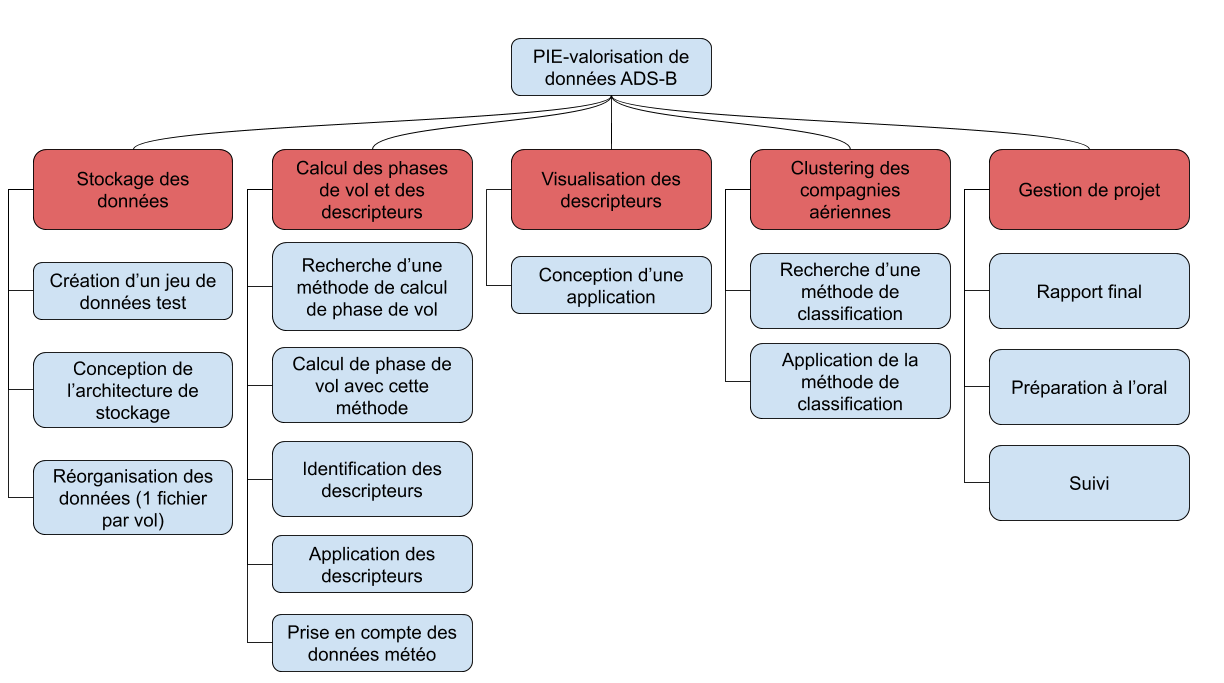
\includegraphics[width=12cm]{WBS}
	\caption{WBS}
	\label{fig:wbs}
\end{figure}
 
\section*{Livrables et critères d'acceptabilité}
\addcontentsline{toc}{section}{Livrables et critères d'acceptabilité}
Les livrables ainsi que leur critère d'acceptabilité sont présentés ci-dessous:
\begin{itemize}
	\item un plan de développement cohérent
	\item un compte-rendu répondant au problème initialement formulé par le client
	\item une soutenance PIE présentant le projet et son déroulement
	\item les codes sources commentés et facilement utilisable par le client
\end{itemize}

%%% Local Variables: 
%%% mode: latex
%%% TeX-master: "isae-report-template"
%%% End: 